\documentclass[10pt,border=0.5pt]{standalone}
\usepackage[T1]{fontenc}
\usepackage{times}
\usepackage{textcomp}
\usepackage{amsmath,amssymb,pifont,bm}
\usepackage{tikz}
\usetikzlibrary{positioning,arrows.meta,calc,fit,backgrounds}
% Shared figure palette (validated categorical slots 1-3 + neutrals)
\definecolor{cFwd}{HTML}{2A78D6}      % GivenRL / forward path (slot 1, blue)
\definecolor{cWrong}{HTML}{EB6834}    % agreement rewards / wrong answer (slot 2, orange)
\definecolor{cInv}{HTML}{1BAF7A}      % inverse path / exact labels (slot 3, aqua)
\definecolor{cInvDark}{HTML}{0F7A53}  % aqua text-safe step
\definecolor{cFwdDark}{HTML}{1C5CAB}  % blue text-safe step
\definecolor{cWrongDark}{HTML}{B8461C}
\definecolor{cInk}{HTML}{2B2B2B}
\definecolor{cMuted}{HTML}{6E6D68}
\definecolor{cRule}{HTML}{C9C8C2}
\definecolor{cPanel}{HTML}{F6F5F2}
\colorlet{cFwdBg}{cFwd!9!white}
\colorlet{cInvBg}{cInv!10!white}
\colorlet{cWrongBg}{cWrong!10!white}

\newcommand{\given}[1]{{\setlength{\fboxsep}{0.5pt}\colorbox{cInv!22!white}{#1}}}
\newcommand{\gmask}{{\setlength{\fboxsep}{0.5pt}\colorbox{cInv!22!white}{$\bm{z}$}}}
\newcommand{\ind}{\mathbf{1}}
\begin{document}
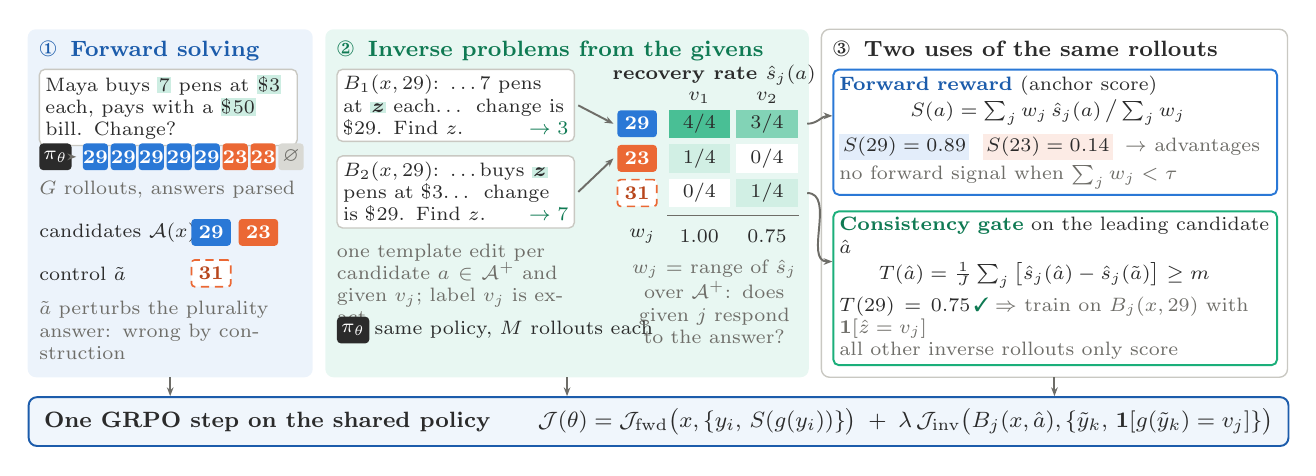
\begin{tikzpicture}[
  font=\scriptsize, text=cInk, line join=round,
  box/.style={draw=cRule, rounded corners=2pt, fill=white, inner sep=2.2pt, align=left, line width=0.5pt},
  tok/.style={rounded corners=1.2pt, minimum width=0.36cm, minimum height=0.34cm, inner sep=0pt, font=\scriptsize\bfseries},
  ctl/.style={tok, draw=cWrong, densely dashed, fill=white, text=cWrongDark, line width=0.6pt},
  arr/.style={-{Stealth[length=3.2pt]}, line width=0.7pt, draw=cMuted},
  title/.style={font=\footnotesize\bfseries, anchor=north west, inner sep=0pt},
  note/.style={font=\scriptsize, text=cMuted, inner sep=0pt},
  pol/.style={rounded corners=1.5pt, fill=cInk, text=white, font=\scriptsize\bfseries, inner sep=1.5pt, minimum height=0.34cm},
]
\useasboundingbox (0,0.02) rectangle (16,-5.32);

%==================== stage frames ====================
\fill[cFwdBg, rounded corners=3pt] (0,0) rectangle (3.62,-4.42);
\fill[cInvBg, rounded corners=3pt] (3.78,0) rectangle (9.92,-4.42);
\draw[cRule, rounded corners=3pt, line width=0.5pt, fill=white] (10.08,0) rectangle (16,-4.42);

%==================== (1) forward ====================
\node[title, text=cFwdDark] at (0.14,-0.14) {\ding{172}\, Forward solving};
\node[box, anchor=north west, text width=3.12cm] (x) at (0.14,-0.5)
  {Maya buys \given{7} pens at \given{\$3} each, pays with a \given{\$50} bill. Change?};
\node[pol, anchor=west] (p1) at (0.14,-1.62) {$\pi_\theta$};
\foreach \i in {0,...,4} {\node[tok, fill=cFwd, text=white, minimum width=0.32cm] at ({0.86+\i*0.355}, -1.62) {29};}
\foreach \i in {5,6} {\node[tok, fill=cWrong, text=white, minimum width=0.32cm] at ({0.86+\i*0.355}, -1.62) {23};}
\node[tok, fill=cRule!70, text=cMuted, minimum width=0.32cm] at ({0.86+7*0.355}, -1.62) {$\varnothing$};
\draw[arr] (p1.east) -- ++(0.05,0);
\node[note, anchor=north west] at (0.14,-1.92) {$G$ rollouts, answers parsed};

\node[note, anchor=west, text=cInk] at (0.14,-2.58) {candidates $\mathcal A(x)$};
\node[tok, fill=cFwd, text=white, minimum width=0.5cm] at (2.33,-2.58) {29};
\node[tok, fill=cWrong, text=white, minimum width=0.5cm] at (2.93,-2.58) {23};
\node[note, anchor=west, text=cInk] at (0.14,-3.1) {control $\tilde a$};
\node[ctl, minimum width=0.5cm] at (2.33,-3.1) {31};
\node[note, anchor=north west, text width=3.35cm] at (0.14,-3.45) {$\tilde a$ perturbs the plurality answer: wrong by construction};

%==================== (2) inverse problems ====================
\node[title, text=cInvDark] at (3.92,-0.14) {\ding{173}\, Inverse problems from the givens};
\node[box, anchor=north west, text width=2.86cm] (b1) at (3.92,-0.5)
  {$B_1(x,29)$: \dots{}7 pens at \gmask{} each\dots{} change is \$29. Find $z$.\hfill{\color{cInvDark}$\to3$}};
\node[box, anchor=north west, text width=2.86cm] (b2) at (3.92,-1.6)
  {$B_2(x,29)$: \dots{}buys \gmask{} pens at \$3\dots{} change is \$29. Find $z$.\hfill{\color{cInvDark}$\to7$}};
\node[note, anchor=north west, text width=3.0cm] at (3.92,-2.72) {one template edit per candidate $a\in\mathcal A^{+}$ and given $v_j$; label $v_j$ is exact};
\node[pol, anchor=west] (p2) at (3.92,-3.82) {$\pi_\theta$};
\node[note, anchor=west, text=cInk] at (4.4,-3.82) {same policy, $M$ rollouts each};

% recovery matrix
\def\cw{0.86}\def\ch{0.44}
\coordinate (M0) at (8.1,-0.98);
\node[font=\scriptsize\bfseries, anchor=south, inner sep=0pt] at ($(M0)+(0.62,0.26)$) {recovery rate $\hat s_j(a)$};
\node[font=\scriptsize, anchor=south, inner sep=1pt] at ($(M0)+(0.5*\cw,0)$) {$v_1$};
\node[font=\scriptsize, anchor=south, inner sep=1pt] at ($(M0)+(1.5*\cw,0)$) {$v_2$};
\foreach \r/\sa/\sb/\fa/\fb in {0/{4/4}/{3/4}/80/55, 1/{1/4}/{0/4}/20/0, 2/{0/4}/{1/4}/0/20} {
  \fill[cInv!\fa!white] ($(M0)+(0.04,-\r*\ch-0.04)$) rectangle ($(M0)+(\cw-0.04,-\r*\ch-\ch+0.04)$);
  \fill[cInv!\fb!white] ($(M0)+(\cw+0.04,-\r*\ch-0.04)$) rectangle ($(M0)+(2*\cw-0.04,-\r*\ch-\ch+0.04)$);
  \node[font=\scriptsize] at ($(M0)+(0.5*\cw,-\r*\ch-0.5*\ch)$) {\sa};
  \node[font=\scriptsize] at ($(M0)+(1.5*\cw,-\r*\ch-0.5*\ch)$) {\sb};
}
\node[tok, fill=cFwd, text=white, minimum width=0.5cm] at ($(M0)+(-0.36,-0.5*\ch)$) {29};
\node[tok, fill=cWrong, text=white, minimum width=0.5cm] at ($(M0)+(-0.36,-1.5*\ch)$) {23};
\node[ctl, minimum width=0.5cm] at ($(M0)+(-0.36,-2.5*\ch)$) {31};
\draw[cMuted, line width=0.4pt] ($(M0)+(0.02,-3*\ch-0.07)$) -- ++(2*\cw-0.04,0);
\node[font=\scriptsize, anchor=east, inner sep=0pt] at ($(M0)+(-0.12,-3*\ch-0.33)$) {$w_j$};
\node[font=\scriptsize] at ($(M0)+(0.5*\cw,-3*\ch-0.33)$) {1.00};
\node[font=\scriptsize] at ($(M0)+(1.5*\cw,-3*\ch-0.33)$) {0.75};
\node[note, anchor=north, text width=2.4cm, align=center] at ($(M0)+(0.62,-3*\ch-0.62)$) {$w_j$ = range of $\hat s_j$ over $\mathcal A^{+}$: does given $j$ respond to the answer?};
\draw[arr] ($(b1.east)+(0.04,0)$) -- ($(M0)+(-0.66,-0.5*\ch)$);
\draw[arr] ($(b2.east)+(0.04,0)$) -- ($(M0)+(-0.66,-1.5*\ch)$);

%==================== (3) two uses ====================
\node[title] at (10.22,-0.14) {\ding{174}\, Two uses of the same rollouts};
\node[box, anchor=north west, text width=5.48cm, draw=cFwd, line width=0.7pt] (fr) at (10.22,-0.5)
  {\textbf{\color{cFwdDark}Forward reward} (anchor score)\\[1.5pt]
   \hspace*{0.9cm}$S(a)=\sum_j w_j\,\hat s_j(a)\,\big/\sum_j w_j$\\[2pt]
   {\setlength{\fboxsep}{1.2pt}\colorbox{cFwd!13}{$S(29)=0.89$}\; \colorbox{cWrong!13}{$S(23)=0.14$}}\;\;{\color{cMuted}$\to$ advantages}\\[1pt]
   {\color{cMuted}no forward signal when $\sum_j w_j<\tau$}};
\node[box, anchor=north west, text width=5.48cm, draw=cInv, line width=0.7pt] (gt) at (10.22,-2.3)
  {\textbf{\color{cInvDark}Consistency gate} on the leading candidate $\hat a$\\[1.5pt]
   \hspace*{0.5cm}$T(\hat a)=\tfrac1J\sum_j\big[\hat s_j(\hat a)-\hat s_j(\tilde a)\big]\ge m$\\[2pt]
   $T(29)=0.75$\,{\color{cInvDark}\ding{51}}\;{\color{cMuted}$\Rightarrow$ train on $B_j(x,29)$ with $\ind[\hat z=v_j]$}\\
   {\color{cMuted}all other inverse rollouts only score}};
\draw[arr] ($(M0)+(2*\cw+0.08,-0.5*\ch)$) to[out=0,in=180] (fr.west |- 0,-1.1);
\draw[arr] ($(M0)+(2*\cw+0.08,-2.5*\ch)$) to[out=0,in=180] (gt.west |- 0,-2.95);

%==================== update bar ====================
\node[draw=cFwdDark, fill=cFwd!7, rounded corners=3pt, line width=0.7pt, minimum width=16cm, minimum height=0.62cm, anchor=north west, align=center] (up) at (0,-4.66)
  {\footnotesize\textbf{One GRPO step on the shared policy}\qquad
   $\mathcal J(\theta)=\mathcal J_{\mathrm{fwd}}\big(x,\{y_i,\,S(g(y_i))\}\big)\;+\;\lambda\,\mathcal J_{\mathrm{inv}}\big(B_j(x,\hat a),\{\tilde y_k,\,\ind[g(\tilde y_k)=v_j]\}\big)$};
\draw[arr] (1.81,-4.42) -- (1.81,-4.66);
\draw[arr] (6.85,-4.42) -- (6.85,-4.66);
\draw[arr] (13.04,-4.42) -- (13.04,-4.66);
\end{tikzpicture}
\end{document}
